\chapter{Mathematical optimization}\label{optimization}

Mathematical optimization, also known as mathematical programming, is a broad field that covers various disciplines, including linear and nonlinear optimization, convex programming, integer programming, and more. The goal of this chapter is to summarize the key concepts and techniques relevant to the scope of this work. Specifically, we will focus on methods for solving optimization problems with constraints and those where the objective function is generally unknown and its evaluation is computationally expensive. Classic methods applicable to unconstrained optimization, such as the Davidon-Fletcher-Powell \cite{Fletcher1963} and Broyden-Fletcher-Goldfarb-Shanno \cite{broyden1970} algorithms, while fundamental, fall outside the scope of this work and details on these methods can be found for instance in \cite{Bert}.

This chapter will focus on methods that address the specific challenges posed by constrained and generally unknown objective functions. First, a general optimization problem is defined, followed by an introduction to basic techniques for solving constrained problems. Next, black-box optimization methods are discussed. Finally, the proposed optimization framework used in this work is presented.

\section{General optimization problem}

Let $m, n, q \in \mathbb{N}$. Define the continuous functions $f : \mathbf{D} \rightarrow \mathbb{R}$, $ \vec{g} : \mathbf{D} \rightarrow \mathbb{R}^m$, $ \vec{h} : \mathbf{D} \rightarrow \mathbb{R}^q $, where $ \mathbf{D} = \mathrm{Dom} \, (f) \cap \mathrm{Dom} \, (\vec{g}) \cap \mathrm{Dom} \, (\vec{h})$, i.e., $ \mathbf{D} $ is the intersection of the domains of the given functions. Next, define the set

\begin{equation}\label{eq:feasible solution}
	\mathbf{X} = \big\{ \vec{x} \in \mathbf{D} \subseteq \mathbb{R}^n \ | \ \vec{g} (\vec{x}) \leq \vec{0} \wedge \vec{h} (\vec{x}) = \vec{0} \, \big\},
\end{equation}
where the inequality $ \vec{g} \leq \vec{0} $ and equality $ \vec{h} = \vec{0} $ are understood component-wise. The general goal of mathematical optimization is to solve the problem
\begin{equation}\label{eq:basic problem}
	\min_{\vec{x} \in \mathbf{X}} f(\vec{x}).
\end{equation}

The function $f$ being minimized is called the objective function, $\mathbf{D}$ is referred to as the domain of the problem, and $\mathbf{X}$~is called the set of feasible solutions of the problem \cite{Bert}. Note that, henceforth, $f$ denotes only the objective function and not the distribution function discussed in Chapter \ref{lbm}.

When classifying optimization problems, we refer to what are known as constraints. These are determined by the definition of the set $ \mathbf{X} $, i.e., the equality and inequality conditions for the functions $ \vec{g} $~and $ \vec{h} $, and by the domain $ \mathbf{D} $. Constraints defined by $ \vec{g} (\vec{x}) \leq \vec{0} \wedge \vec{h} (\vec{x}) = \vec{0} $ are called explicit constraints, while those determined by the domain $ \mathbf{D} $ are called implicit constraints.
\newpage
The optimal solution of the problem \eqref{eq:basic problem} is denoted by $ \vec{x}^{\star} \in \mathbf{X} $ and is defined as
\begin{equation}
	\vec{x}^{\star} = \operatorname*{argmin}_{\vec{x} \in \mathbf{X}} \, f(\vec{x}).
\end{equation}
Note that the optimal solution may not be unique, and we refer to the set of all optimal solutions as the optimal set. It is also important to recognize that the search for an optimal solution can equivalently be formulated as finding the maximum of the function $ -f$ over the same set $ \mathbf{X}$, enabling the use of the same techniques for solving maximization problems \cite{Bert, non-linear-textbook}.
\section{Solving constrained problems}\label{constrained}
We will now consider the problem \ref{eq:basic problem}, where the set of admissible solutions is given by \ref{eq:admissible solution}. In this section, we describe how to generally solve this problem by converting it into a sequence of unconstrained optimization problems. There exist several other methods for solving constrained problems, but here we will focus on the penalty and the barrier methods.

\subsection{Penalty methods}\label{penalty method}
As mentioned earlier, penalty methods convert constrained optimization problems into unconstrained ones. The fundamental principle of penalty methods is to incorporate the conditions that define the set of admissible solutions by adding a penalty term to the objective function, which reflects the degree of violation of those conditions \cite{Bert}. The penalty function is defined as a continuous scalar function on $ \mathbb{R}^n $ that satisfies

\begin{align}
	\begin{split}
		p(\vec{x}) &= 0, \ \ \forall \vec{x} \in \mathbf{X},\\[6pt]
		p(\vec{x}) &> 0, \ \ \text { otherwise. }
	\end{split}
\end{align}
A typical choice for the penalty function is, e.g.,
\begin{equation}\label{eq:penalty function}
	p (\vec{x}) = \sum_{j=1}^{m} \left( \, \max  \left\{ \, g_j (\vec{x}), 0 \, \right\} \, \right)^2 + \sum_{j=1}^{q} h_j (\vec{x})^2.
\end{equation}
Using the penalty function $ p $, we construct the modified objective function
\begin{equation}\label{eq:cost function with penalty}
	\phi (\vec{x}, r) = f (\vec{x}) + r p(\vec{x}),
\end{equation}
where $ r > 0 $ is called the penalty coefficient \cite{Bert}. From the definition of the penalty function, it can be seen that the values of the modified objective function $ \phi (\vec{x}, r)$ differ from the original function $ f $ only for such $ \vec{x} $ that violate the specified condition.

To solve the constrained problem, we iteratively construct a new term in an increasing sequence of penalty coefficients $ r_1, r_2, \dots$, for which we solve the unconstrained optimization problem for the modified function $ \phi (\vec{x}, r_k)$. The optimal solution $ \vec{x}_k $ of this unconstrained problem is then used as the starting point for the next iteration. This process is repeated until the condition $ r_k p(\vec{x}_k) < \varepsilon$ for some $ \varepsilon > 0$ is satisfied. When this condition is met, $ \vec{x}_k $ can be considered a sufficiently accurate approximation of the solution to the constrained problem. It should be noted that penalty methods allow searching for an optimal solution outside the set of admissible solutions during the iterations \cite{non-linear-textbook}, and thus are categorized as exterior point methods. A key assumption of penalty methods is that the domain of the problem satisfies $ \mathbf{D} = \mathbb{R}^n $.

The construction of the sequence of penalty parameters and the principle of the penalty method are illustrated in Figure~\ref{fig:penalty} on a trivial example of minimizing the function $ f(x) = 0.5x $ with the constraint $ g(x) = 4 - x \leq 0 $. The modified objective function in this case takes the form
\begin{equation}
	\phi (x, r) = 0.5x + r \left(\max  \left\{ \,  4-x, 0 \right\}\right)^2.
\end{equation}
\begin{figure}[H]
	\vspace{-2.25cm}
	\centering
	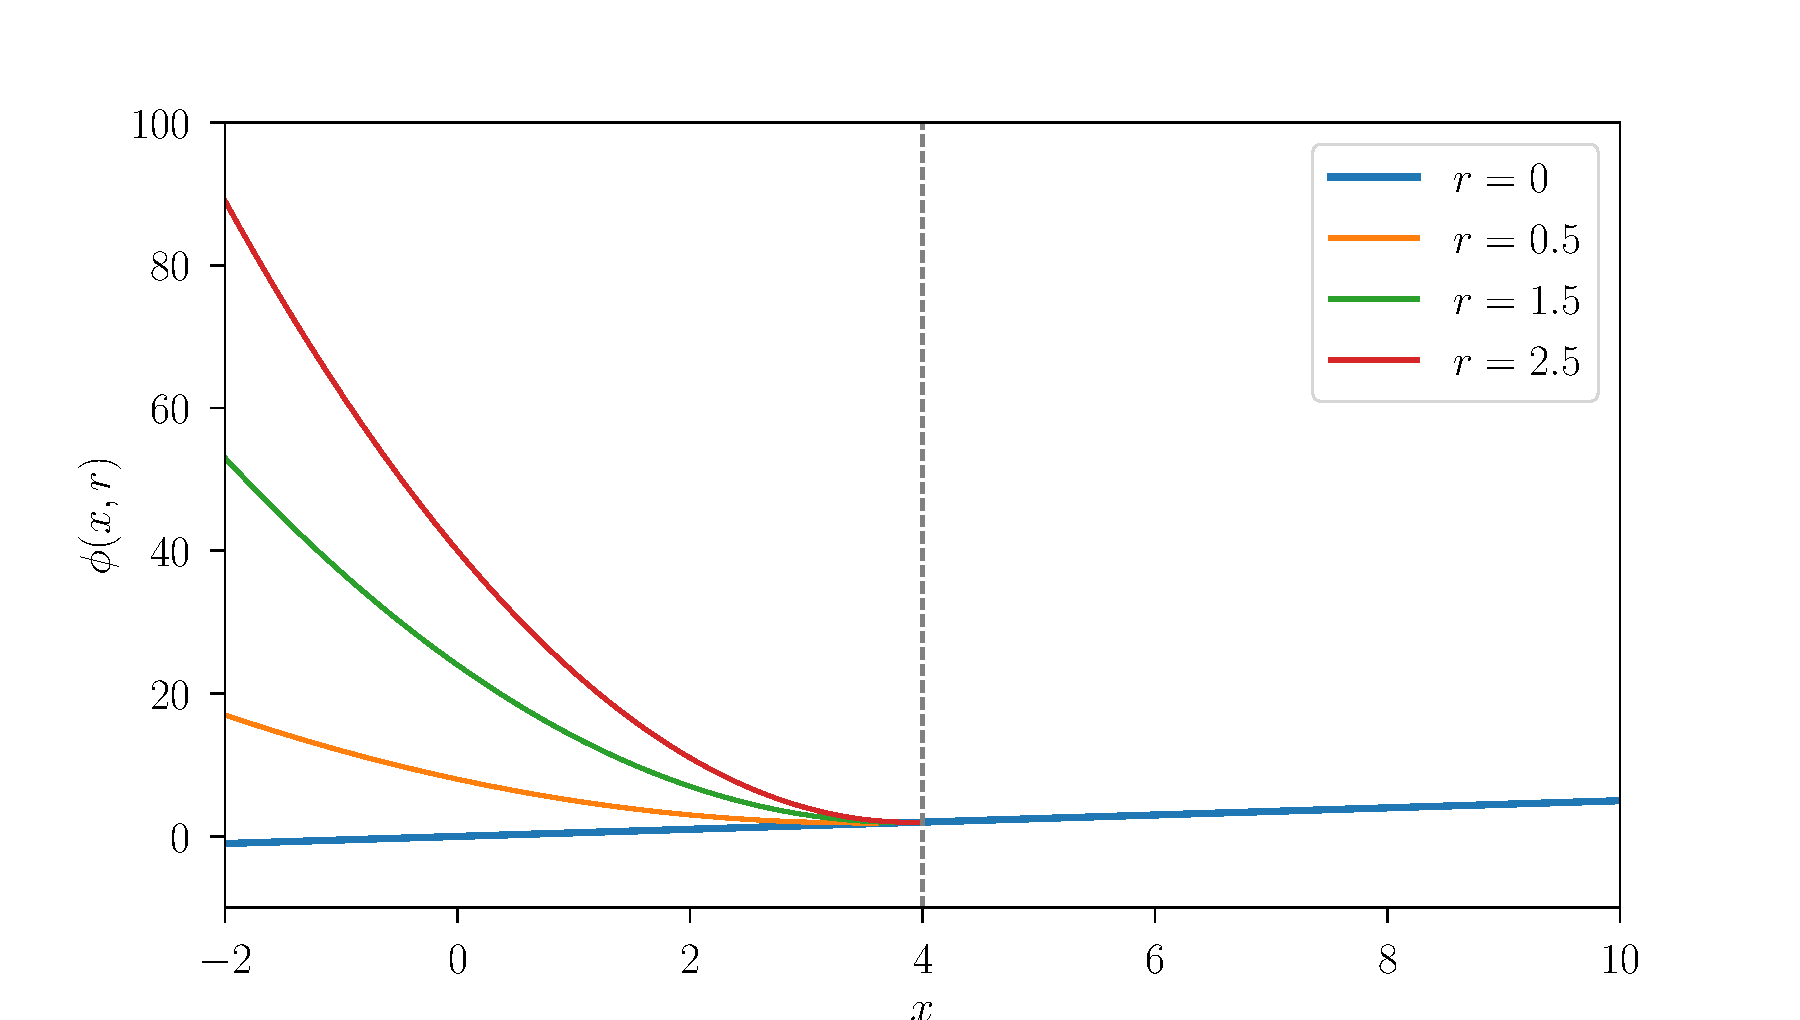
\includegraphics[width=0.9\textwidth]{figures/penalty.pdf}
%	\vspace{0.2cm}
	\caption{An illustration of the penalty method applied to minimizing the function $ f(x) = 0.5x $ with the constraint $ g(x) = 4 - x \leq 0 $. Different shapes of the modified objective function $ \phi (x, r) $ depending on the value of the penalty parameter $ r $ are distinguished by color. The condition defining the set of admissible solutions is indicated by the gray dashed line. The set of admissible solutions lies in the half-plane to the right of this gray dashed line.}
	\label{fig:penalty}
\end{figure}


\subsection{Barrier method}\label{barrier method}
The barrier method operates on a principle similar to that of the penalty method, but its main difference is that, during the iterative process of finding an optimal solution to a constrained problem, it ensures that the solution estimates always remain within the interior of the feasible set, which is defined as
\begin{equation}
	\mathbf{X}^{\mathrm{o}} = \left\{ \vec{x} \in \mathbf{D} \subseteq \mathbb{R}^n \ \middle| \ \vec{g}(\vec{x}) < \vec{0} \right\}.
\end{equation}
Methods that satisfy this condition are generally referred to as interior-point methods \cite{non-linear-textbook}.

As with penalty methods, we account for the conditions defining the feasible set by adding a new term to the objective function, which reflects the degree to which these conditions are violated. The barrier function $ B $ is a continuous scalar function on $ \mathbf{X}^{\mathrm{o}} $ that satisfies the condition
\begin{equation}
	(\exists j \in \{1,2,\dots,m\})(\lim\limits_{\substack{\vec{x} \to \vec{y} \\ \mathbf{X}^{\mathrm{o}}}} g_j (\vec{x}) = 0) \Rightarrow \lim\limits_{\substack{\vec{x} \to \vec{y} \\ \mathbf{X}^{\mathrm{o}}}} B (\vec{x}) = + \infty.
\end{equation}
A typical choice for the barrier function is the logarithmic barrier function
\begin{equation}\label{eq:log barrier function}
	B (\vec{x}) = -\sum_{j=1}^{m} \ln \left( - g_j (\vec{x}) \right),
\end{equation}
or alternatively, the reciprocal barrier function
\begin{equation}\label{eq:reciprocal barrier function}
	B (\vec{x}) = -\sum_{j=1}^{m} \frac{1}{g_j (\vec{x})}.
\end{equation}
Using the barrier function $ B $, similar to the penalty methods, we construct the modified objective function
\begin{equation}\label{eq:cost function with barrier}
	\phi (\vec{x}, r) = f (\vec{x}) + r B(\vec{x}),
\end{equation}
where $ r > 0 $ is a chosen parameter \cite{non-linear-textbook}.

To solve the constrained problem using the barrier method, at each iteration we construct a new term in a strictly decreasing sequence of positive parameters $ r_1, r_2, \dots$, for which we solve the unconstrained optimization problem for the modified function $ \phi (\vec{x}, r_k)$. The vector $ \vec{x}_k  = \operatorname*{argmin}_{\vec{x} \in \mathbf{X}^\mathrm{o}} (f(\vec{x}) + r_k B(\vec{x})) $, obtained by optimizing the unconstrained problem, is used as the starting point for the next iteration. This process is repeated until the condition $ r_k < \varepsilon$ for some chosen $ \varepsilon > 0$ is satisfied, at which point $ \vec{x}_k $ is considered a sufficient approximation to the solution of the constrained problem \cite{non-linear-textbook}.

The construction of the parameter sequence $ (r_k)_{k \in \mathbb{N}} $ and the principle of the barrier method are illustrated in Fig.~\ref{fig:barrier} using the example of minimizing the function $ f(x) = 0.5x $ with the constraint $ g(x) = 4 - x \leq 0 $ and the choice of the reciprocal barrier function. The modified objective function in this case is
\begin{equation}
	\phi (x, r) = 0.5x - \frac{r}{4-x}.
\end{equation}

\begin{figure}[H]
	\centering
	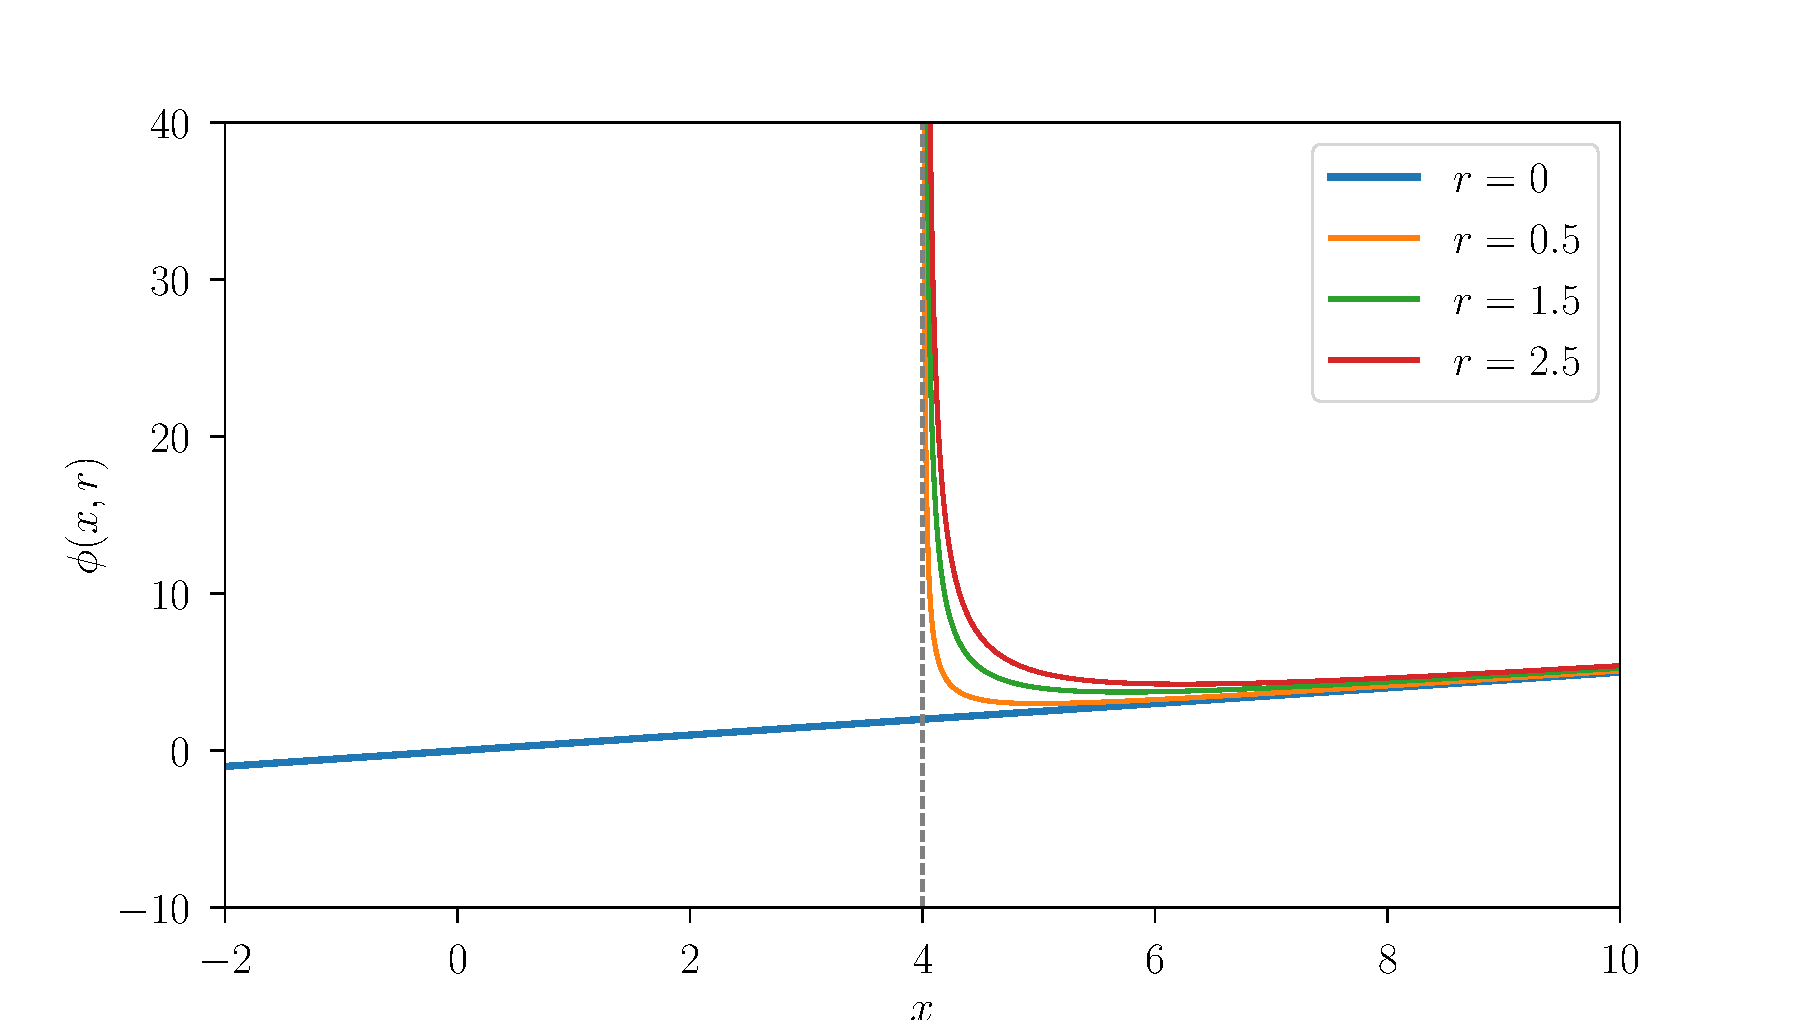
\includegraphics[width=0.9\textwidth]{figures/barrier.pdf}
	\caption{An illustration of the barrier method applied to minimizing the function $ f(x) = 0.5x $ with the constraint $ g(x) = 4 - x \leq 0 $. Different shapes of the modified objective function $ \phi (x, r) $ depending on the value of the barrier parameter $ r $ are distinguished by color. The condition defining the set of feasible solutions is indicated by the gray dashed line. The set of feasible solutions lies in the half-plane to the right of this gray dashed line.}
	\label{fig:barrier}
\end{figure}

Finally, we mention the choice of the barrier function $ B_{\infty} $ used to define the so-called extreme barrier function, as the modified objective function is called with this choice \cite{BBO-textbook}. This barrier function mirrors the asymptotic behavior of the aforementioned barrier functions and is given by
\begin{align}
	\begin{split}
		B_{\infty}(\vec{x}) &= 0, \ \ \forall \vec{x} \in \mathbf{X},\\[6pt]
		B_{\infty}(\vec{x}) &= +\infty, \ \ \text{otherwise.}
	\end{split}
\end{align}
The modified objective function (extreme barrier function) is then given by
\begin{align}\label{eq:extreme barrier}
	\begin{split}
		f_{\infty}(\vec{x}) &= f(\vec{x}) , \ \ \forall \vec{x} \in \mathbf{X},\\[6pt]
		f_{\infty}(\vec{x}) &= +\infty, \ \ \text{otherwise.}
	\end{split}
\end{align}
\section{Black-box optimization}\label{black-box}
In practice, we often need to optimize an objective function $f$ whose exact form and derivative are unknown. This is common in numerical simulations, where the function can only be evaluated at specific points. Moreover, evaluating the function at a point may be difficult, time-consuming, or computationally expensive. As a result, standard optimization algorithms are not well-suited for these problems.

The discipline that deals with problems where the objective function (or constraints) is given by a so-called black-box\footnote{In programming, a black-box refers to a system whose internal mechanisms are unknown to the user. This means that the user generally has access only to the system’s input and output \cite{BBO-textbook}.}, is called black-box optimization (hereafter referred to as BBO). In BBO, it is typically not assumed that the objective function is continuous or differentiable \cite{BBO-textbook, derivative-free-review, two-decades}.

It is worth noting that in the literature, black-box optimization is often confused with derivative-free optimization (DFO), which encompasses methods and techniques for objective functions whose derivatives are unknown or difficult to compute \cite{BBO-textbook, derivative-free-review, Kramer2011}. These two disciplines share many common characteristics, but they differ primarily in that, within DFO, the formula for calculating the derivative of the objective function may still be known. Furthermore, BBO includes heuristic methods, whereas DFO focuses mainly on methods that can be reliably analyzed mathematically in terms of convergence and stopping criteria, which is often not possible for BBO methods \cite{BBO-textbook}. Therefore, although the terms BBO and DFO are often used interchangeably, in this work, we will treat them as two distinct disciplines \cite{BBO-textbook}.

Additionally, it should be noted that various classifications of methods within BBO can be found in the literature. In this work, we will adhere to the classification presented in \cite{BBO-textbook}, distinguishing between heuristic methods, direct search methods, and methods based on surrogate models. Each of these classes will be briefly described in this section.


\subsection{Heuristic Methods}\label{heuristic}
Heuristic optimization methods often rely on different predefined rules or even trial and error when seeking the solution of an optimization problem. These methods usually do not guarantee optimal solutions, but they are often effective for finding near-optimal results in a reasonable amount of time. Heuristic methods include genetic algorithms, detailed in \cite{BBO-textbook}, along with various other heuristic approaches.

In this section, however, we will focus on a different widely used heuristic method, the Nelder-Mead method, also known as the simplex method\footnote{A simplex in $ \mathbb{R}^n $ is defined as a bounded convex polytope (a generalization of a polyhedron to any dimension) with a non-empty interior and exactly $ n+1 $ vertices \cite{BBO-textbook}.}\footnote{The term "simplex method" more commonly refers to the algorithm used to find the optimal solution in linear programming. This algorithm was developed by George Dantzig \cite{Dantzig1990}.}\cite{Nelder1965}.

The Nelder-Mead method finds a solution to an optimization problem by iteratively constructing simplexes. The process begins by initializing a starting simplex. The objective function is then evaluated at each vertex of this simplex. In each subsequent iteration, the simplex is transformed in order to move closer to the position of the sought stationary point of the objective function. The transformation of the simplex involves manipulating its points using predefined operations -- expansion, reflection, contraction (inner and outer), and shrinking, which are schematically illustrated in Figure~\ref{fig:NM operations}. 

\begin{figure}[H]
	%	\vspace{5mm}
	\centering
	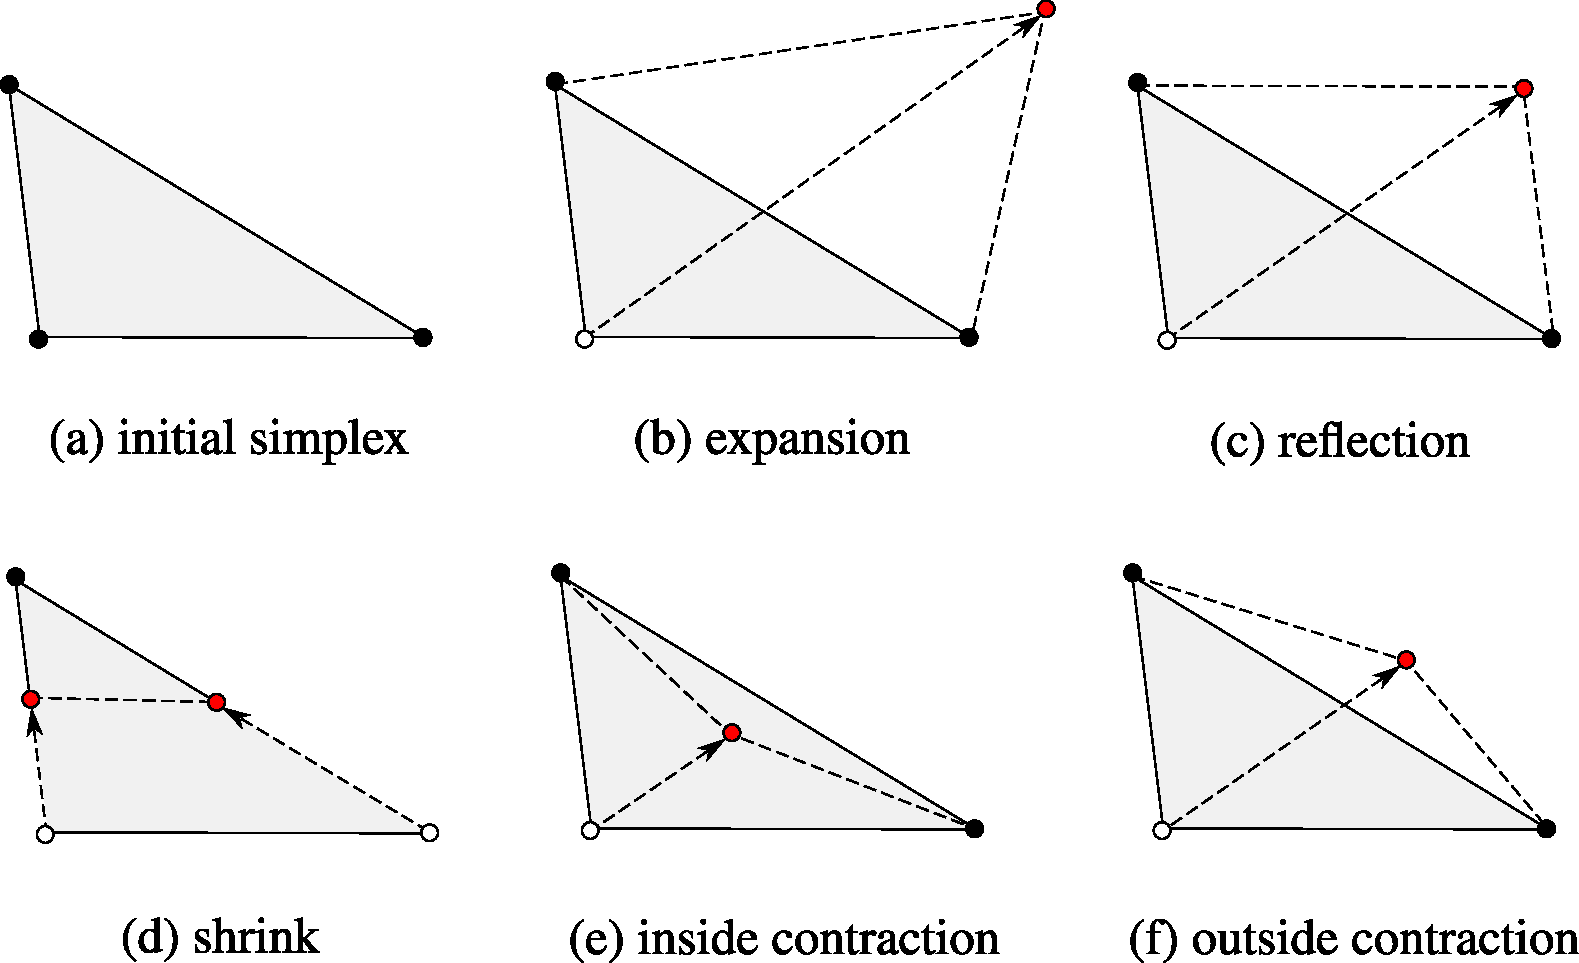
\includegraphics[width=0.96\textwidth]{figures/neldermead.pdf}
	\vspace{2mm}
	\caption{A schematic representation of the operations used to transform simplexes in the Nelder-Mead method. The vertices generated by applying each operation are shown in red. For clarity, the operations are depicted in $ \mathbb{R}^2 $.}
	%	\vspace{2mm}
	\label{fig:NM operations}
\end{figure}

The transformations performed during each iteration are determined by comparing the function values at the vertices of the simplex. The newly formed simplex shares either exactly one vertex or exactly $ n $ vertices with the simplex from the preceding iteration. The algorithm continues to iteratively transform the simplex until a stopping condition (specified by the user) is met \cite{BBO-textbook}. Details of the Nelder-Mead method, including the algorithm's description and the choice of stopping condition, are discussed in \cite{BBO-textbook, derivative-free-review, Nelder1965}. The full Nelder-Mead method algorithm is presented in Algorithm~\ref{neldermead}.

\begin{algorithm}
	\caption{Nelder-Mead algorithm}\label{neldermead}
	\begin{algorithmic}[1]
		\Require Initial simplex $S^0 = \{s^0, s^1, \dots, s^n\}$, function $f: \mathbb{R}^n \to \mathbb{R}$, parameters $\delta^{\text{e}}$, $\delta^{\text{oc}}$, $\delta^{\text{ic}}$, $\gamma$, iteration counter $k \gets 0$
		\Ensure Approximate optimal solution $\vec{x^{\star}}$ for function $f$
		
		\Procedure{Nelder-Mead}{$S^0$}
		\State Reorder $S^k$ so that $f(s^0) \leq f(s^1) \leq \dots \leq f(s^n)$
		\State Set $f^k_{\text{best}} = f(s^0)$
		
		\While{stopping condition not met}
		\Algphase{Reflection}
		\State Compute centroid $x^{\text{c}} = \frac{1}{n} \sum_{i=0}^{n-1} s^i$
		\State Set reflection point $x^{\text{r}} = x^{\text{c}} + (x^{\text{c}} - s^n)$ and compute $f^{\text{r}} = f(x^{\text{r}})$
		\If{$f^k_{\text{best}} \leq f^{\text{r}} < f(s^{n-1})$}
		\State Set $S^{k+1} = \{s^0, s^1, \dots, s^{n-1}, x^{\text{r}}\}$
		\State Increment $k \gets k+1$ and continue
		\EndIf
		
		\Algphase{Expansion}
		\If{$f^{\text{r}} < f^k_{\text{best}}$}
		\State Set expansion point $x^{\text{e}} = x^{\text{c}} + \delta^{\text{e}} (x^{\text{r}} - x^{\text{c}})$ and compute $f^{\text{e}} = f(x^{\text{e}})$
		\If{$f^e < f^r$}
		\State Set $S^{k+1} = \{s^0, s^1, \dots, s^{n-1}, x^\text{e}\}$
		\Else
		\State Set $S^{k+1} = \{s^0, s^1, \dots, s^{n-1}, x^\text{r}\}$
		\EndIf
		\State Increment $k \gets k+1$ and continue
		\EndIf
		
		\Algphase{Contraction}
		\If{$f^\text{r} \geq f(s^n)$}
		\State \textbf{Outside Contraction:} Compute $x^\text{oc} = x^\text{c} + \delta^{\text{oc}}(x^\text{c} - s^n)$ and $f^{\text{oc}} = f(x^{\text{oc}})$
		\If{$f^{\text{oc}} < f(s^n)$}
		\State Set $S^{k+1} = \{s^0, s^1, \dots, s^{n-1}, x^{\text{oc}}\}$
		\Else
		\State \textbf{Shrink:} Set $S^{k+1} = \{s^0, s^0 + \gamma(s^1 - s^0), \dots, s^0 + \gamma(s^n - s^0)\}$
		\EndIf
		\State Increment $k \gets k+1$ and continue
		\Else
		\State \textbf{Inside Contraction:} Compute $x^{\text{ic}} = x^\text{c} + \delta^{\text{ic}}(x^\text{c} - s^n)$ and $f^{\text{ic}} = f(x^{\text{ic}})$
		\If{$f^{\text{ic}} < f(s^n)$}
		\State Set $S^{k+1} = \{s^0, s^1, \dots, s^{n-1}, x^{\text{ic}}\}$
		\Else
		\State Set $S^{k+1} = \{s^0, s^0 + \gamma(s^1 - s^0), \dots, s^0 + \gamma(s^n - s^0)\}$
		\EndIf
		\State Increment $k \gets k+1$ and continue
		\EndIf
		\EndWhile
		\EndProcedure
	\end{algorithmic}
\end{algorithm}
%
The heuristic nature of the Nelder-Mead method stems from the fact that its principle is based on a somewhat random search of the space using predefined rules. Several iterations of space exploration using simplexes, for a specific choice of initial simplex and a specific function, are shown in Figure \ref{fig:NM}. While the convergence of this method has been proven, it is not guaranteed that the method will always converge to a stationary point \cite{BBO-textbook}. It should be noted that the Nelder-Mead method was primarily developed for unconstrained optimization problems, but it can be adapted for constrained optimization problems  \cite{BBO-textbook}.


\begin{figure}[H]
	\vspace{-5mm}
	\begin{subfigure}[b]{0.325\textwidth}
		\centering
		%		trim={<left> <lower> <right> <upper>}
		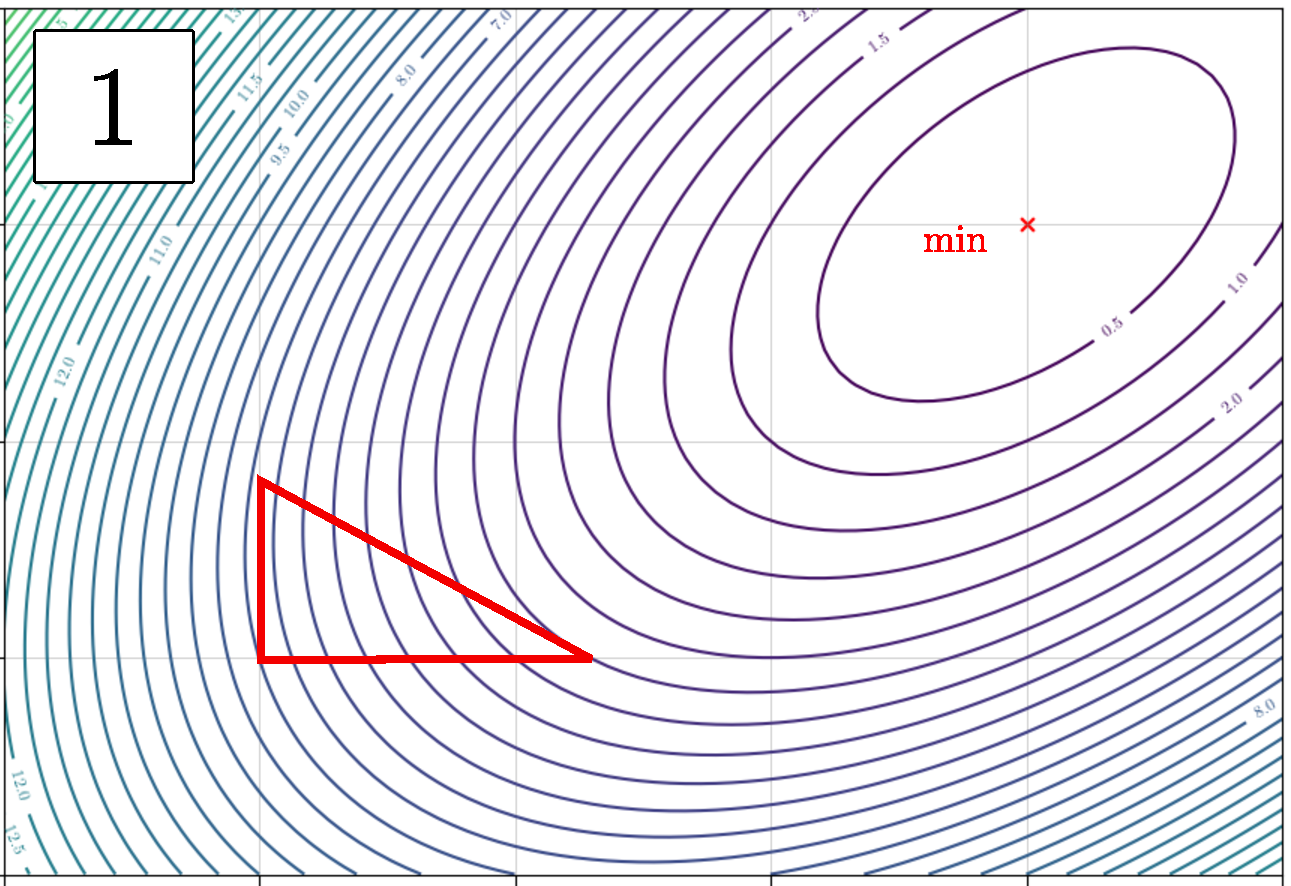
\includegraphics[width=0.96\textwidth, trim={0 0 0 0}, clip]{figures/nelder1.pdf}
	\end{subfigure}
	\begin{subfigure}[b]{0.325\textwidth}
		\centering
		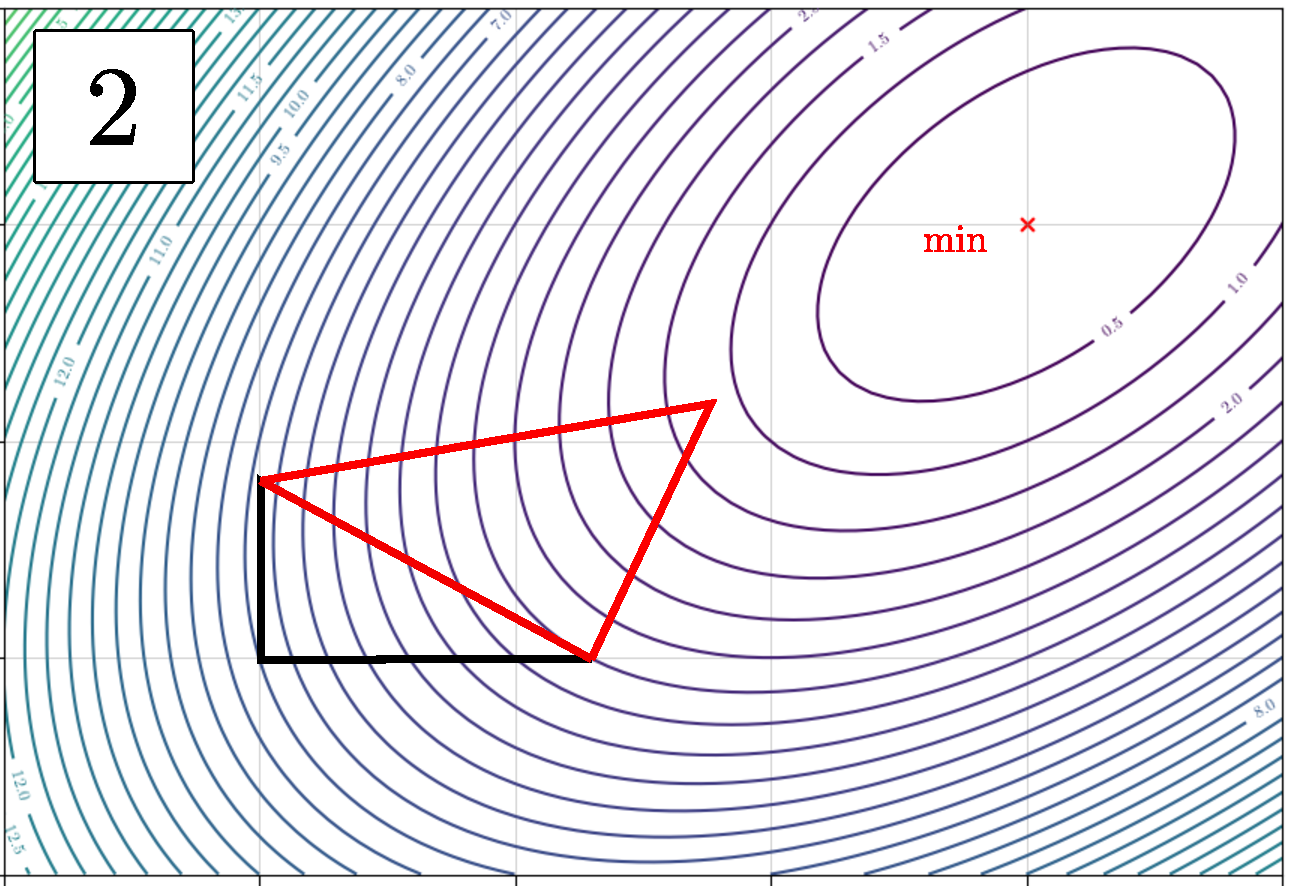
\includegraphics[width=0.96\textwidth, trim={0 0 0 0}]{figures/nelder2.pdf}
	\end{subfigure}
	\vspace{1mm}
	\begin{subfigure}[b]{0.325\textwidth}
		\centering
		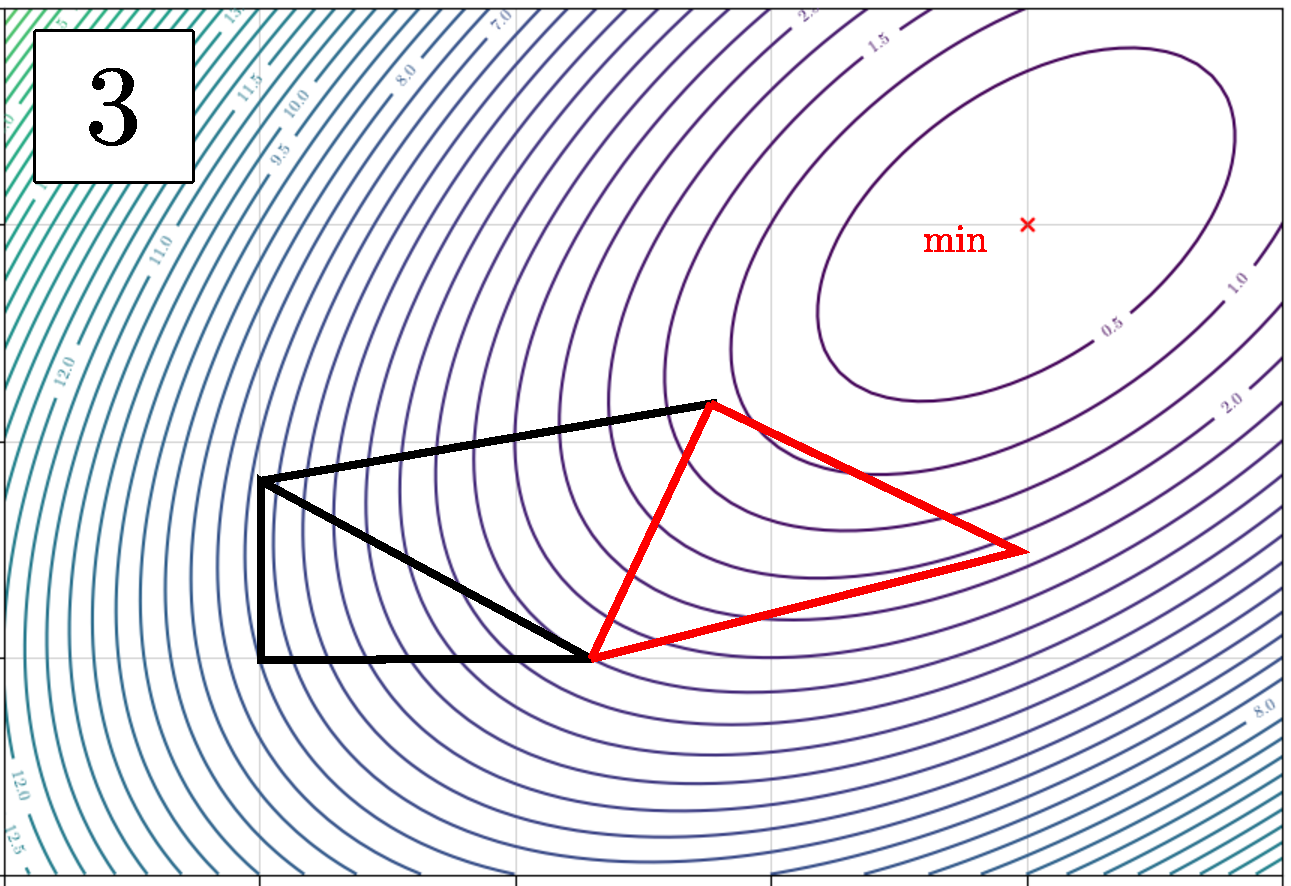
\includegraphics[width=0.96\textwidth, trim={0 0 0 0}]{figures/nelder3.pdf}
	\end{subfigure}
	\vspace{1mm}
	\begin{subfigure}[b]{0.325\textwidth}
		\centering
		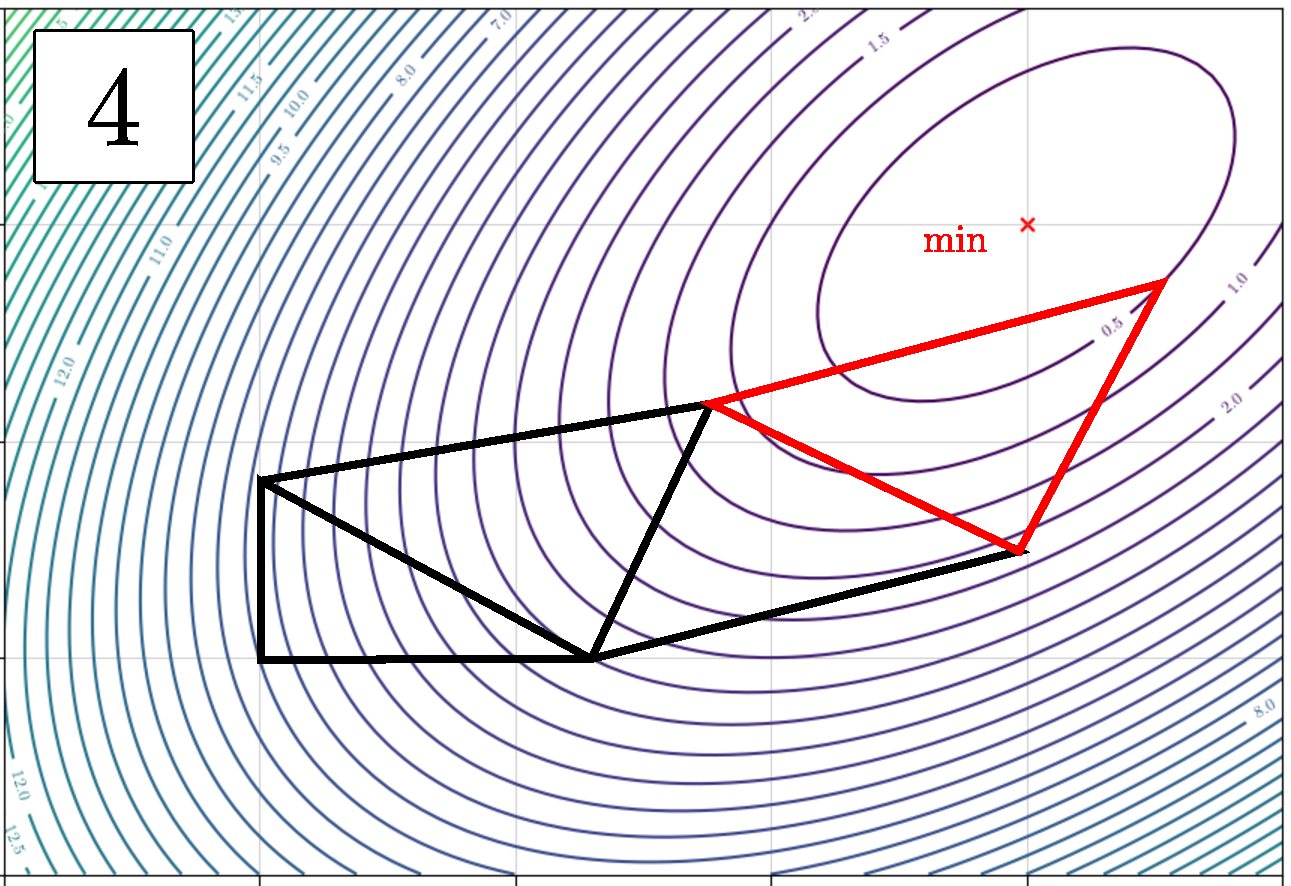
\includegraphics[width=0.96\textwidth, trim={0 0 0 0}]{figures/nelder4.pdf}
	\end{subfigure}
	\begin{subfigure}[b]{0.325\textwidth}
		\centering
		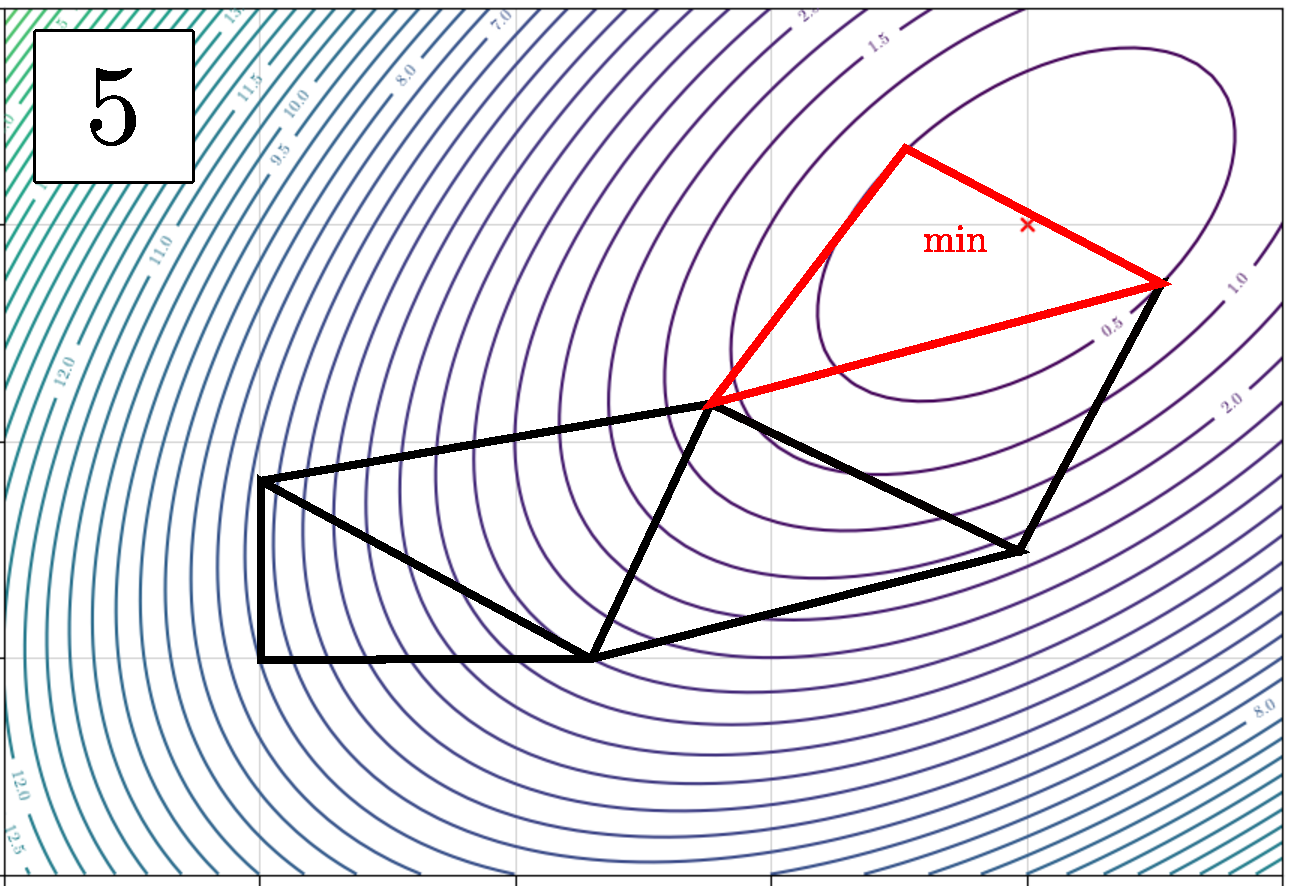
\includegraphics[width=0.96\textwidth, trim={0 0 0 0}]{figures/nelder5.pdf}
	\end{subfigure}
	\begin{subfigure}[b]{0.325\textwidth}
		\centering
		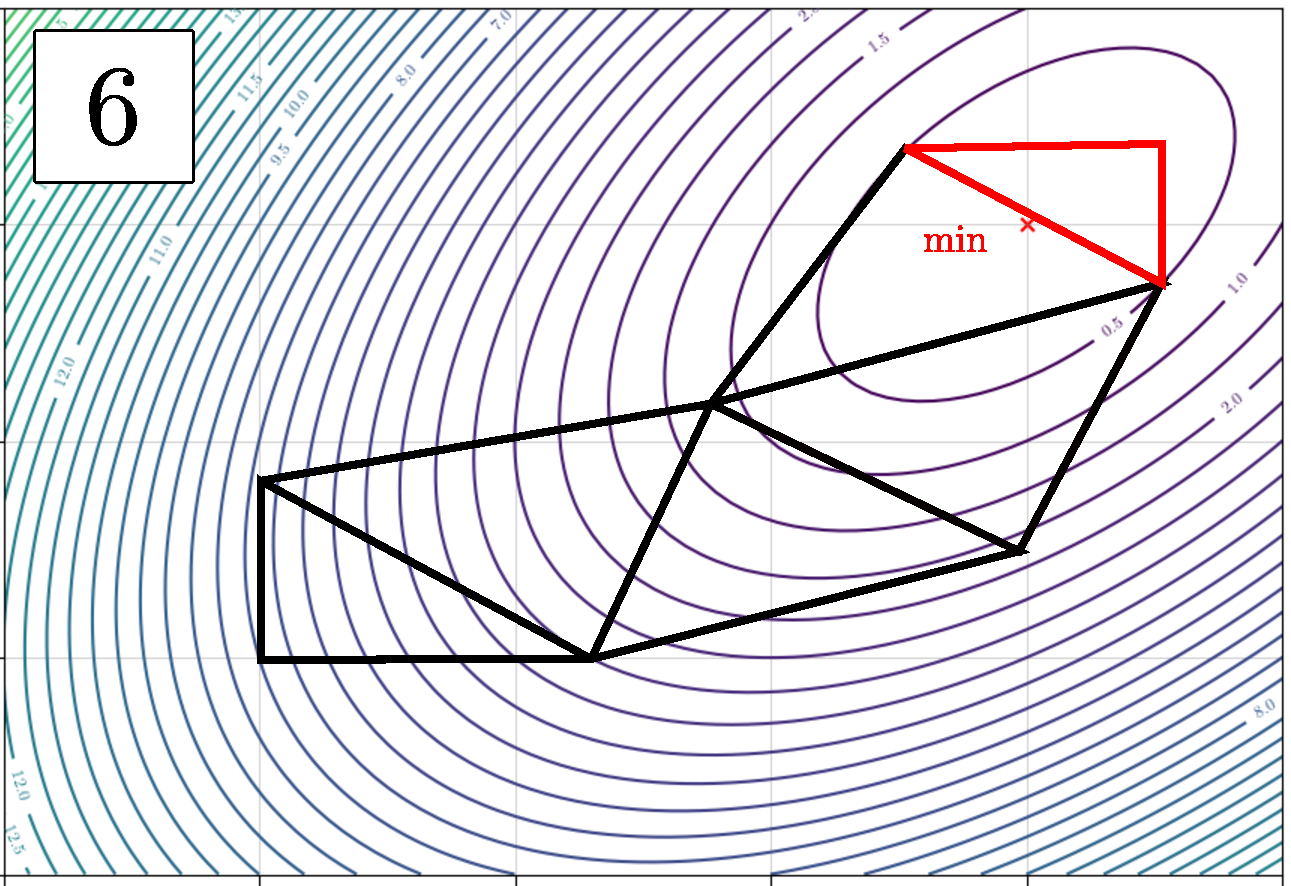
\includegraphics[width=0.96\textwidth, trim={0 0 0 0}]{figures/nelder6.pdf}
	\end{subfigure}
	\centering
	\begin{subfigure}[b]{0.325\textwidth}
		\centering
		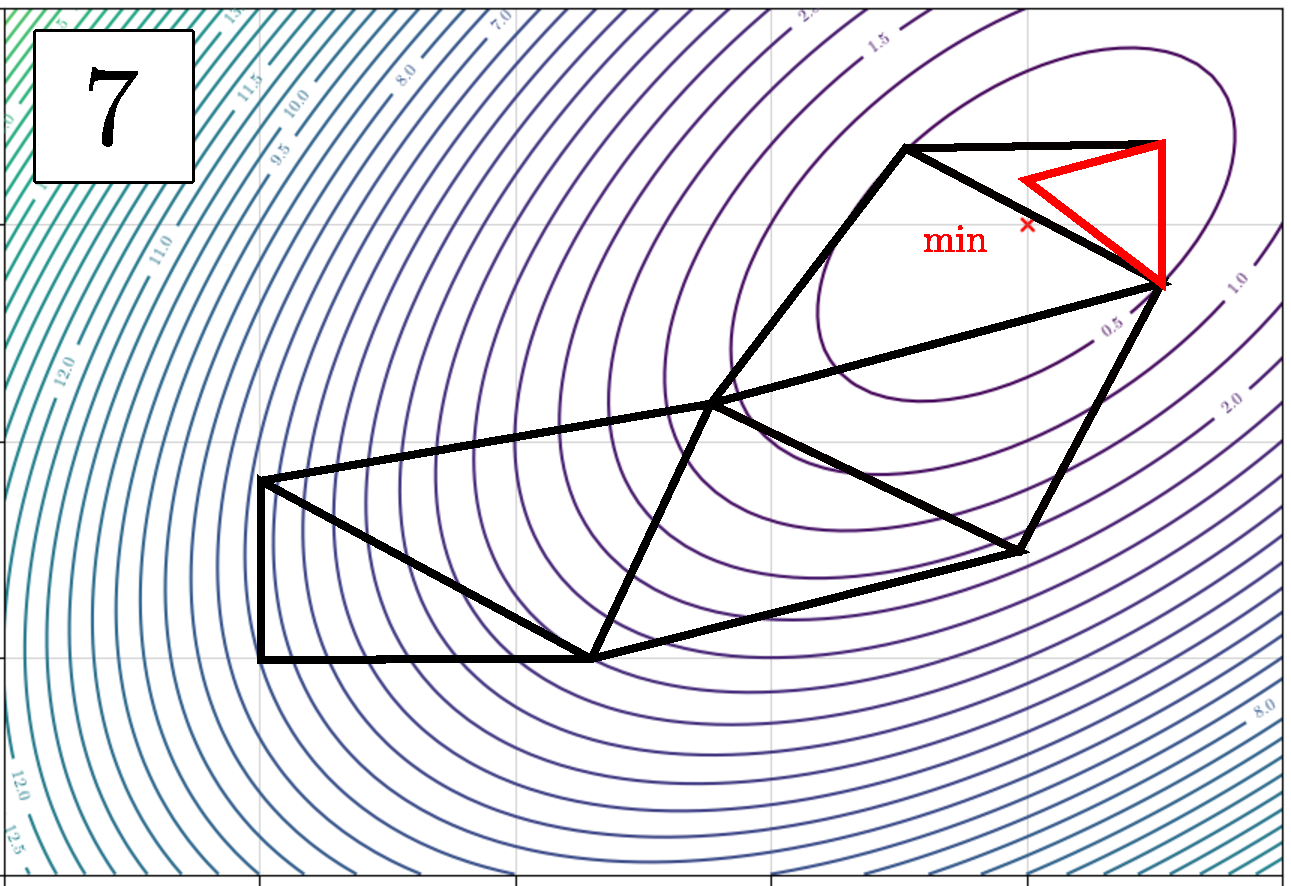
\includegraphics[width=0.96\textwidth, trim={0 0 0 0}]{figures/nelder7.pdf}
	\end{subfigure}
	\begin{subfigure}[b]{0.325\textwidth}
		\centering
		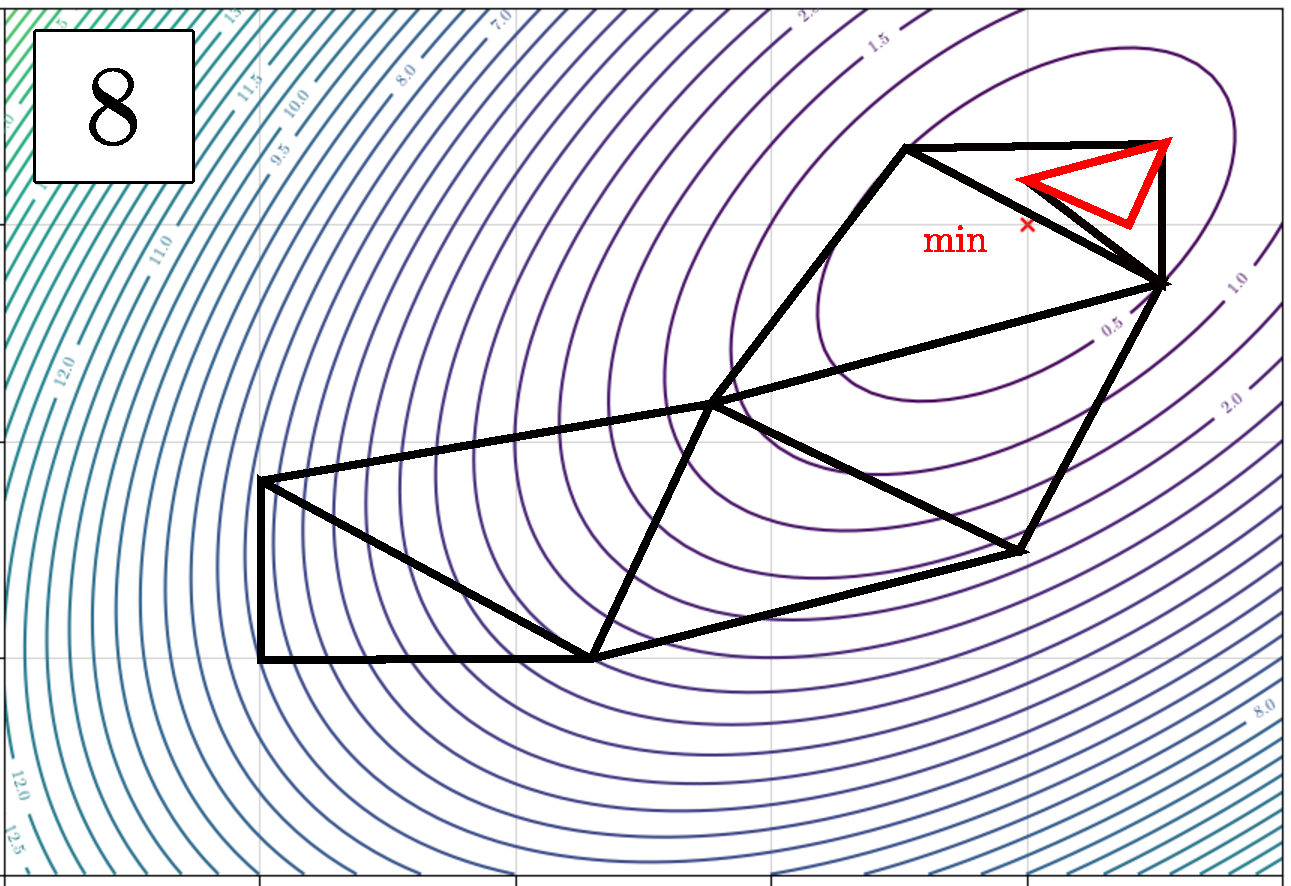
\includegraphics[width=0.96\textwidth, trim={0 0 0 0}]{figures/nelder8.pdf}
	\end{subfigure}
	\begin{subfigure}[b]{0.325\textwidth}
		\centering
		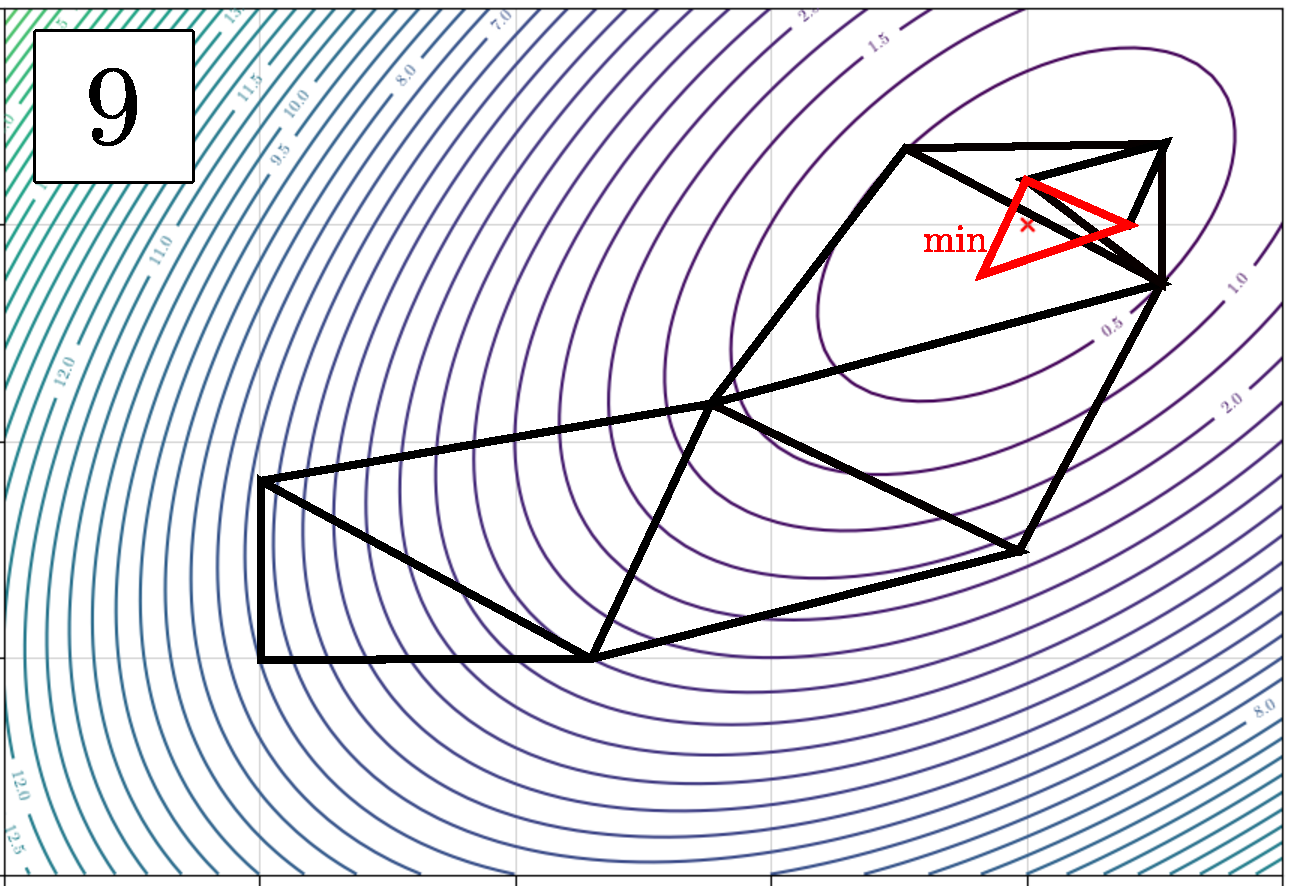
\includegraphics[width=0.96\textwidth, trim={0 0 0 0}]{figures/nelder9.pdf}
	\end{subfigure}
	\begin{center}
		\begin{subfigure}[b]{0.77\textwidth}
			\centering
			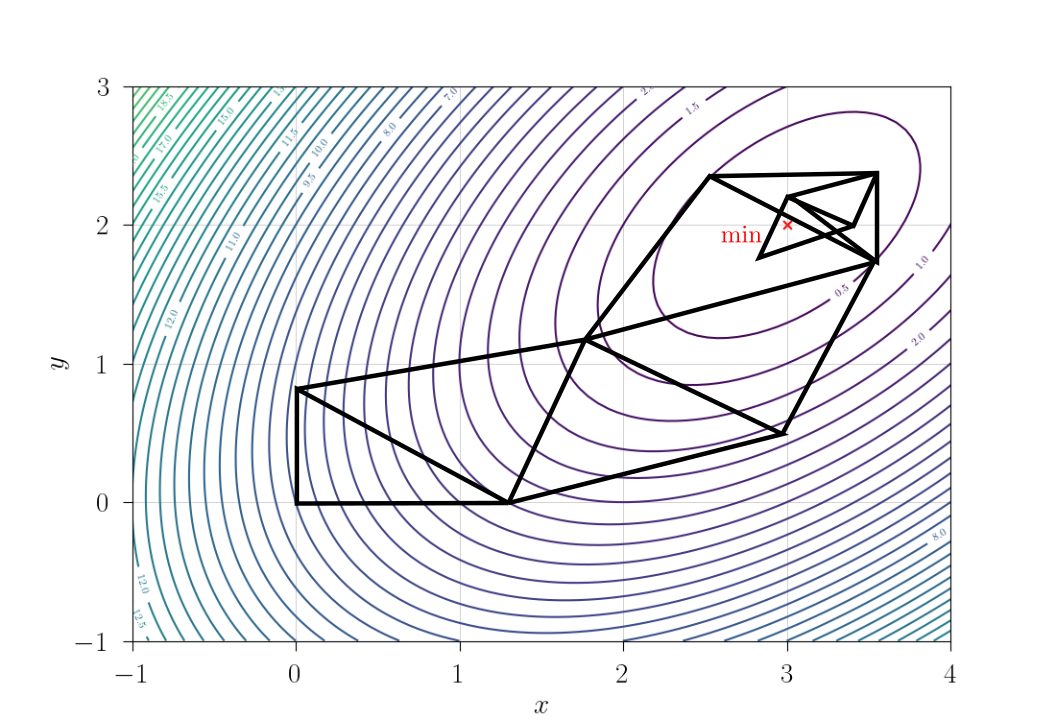
\includegraphics[width=0.985\textwidth, trim={0 6mm 0 7mm}]{figures/nelder.png}
		\end{subfigure}
	\end{center}
	
	\caption{Several iterations of the Nelder-Mead method for a specific choice of the initial simplex when minimizing the function $ x^2 - 4x + y^2 - y - xy + 7 $, with the minimum at the point (3,2) marked by a red cross.}
	\label{fig:NM}
\end{figure}


\subsection{Direct search methods}\label{direct-search}
In this part, we describe the \textit{generalized pattern search} (hereafter GPS) method \cite{Audet2002} and the \textit{mesh adaptive direct search} (hereafter MADS) method \cite{Audet2006}.

To describe the GPS algorithm, it is necessary to define a mesh, which is used to describe the search sets within the GPS algorithm. Let $ \mathbf{G} \in \mathbb{R}^{n \times n} $ be invertible and $ \mathbf{Z} \in \mathbb{Z}^{n \times p} $, $n, p \in \mathbb{N}$. Assume that every vector from $ \mathbb{R}^{n} $ can be expressed as a linear combination of the columns of matrix $ \mathbf{Z} $ (treated as vectors), such that all the coefficients in this linear combination are non-negative. Furthermore, let $ \mathbf{D} = \mathbf{G} \mathbf{Z} $. The mesh $ \mathbf{M} $ generated by $ \mathbf{D} $ centered at point $ \vec{x} $ is defined as
\begin{equation}
	\mathbf{M} = \left\{ \vec{x} + \delta \, \mathbf{D} y \, | \, y \in \mathbb{N}^p \right\},
\end{equation}
where $ \delta $ is called the mesh size parameter \cite{BBO-textbook, Audet2002}. In each iteration of the GPS algorithm, the shape of the mesh generally changes, as it is always centered at the point representing the best estimate in that iteration, and the size of the mesh step also changes. Let $ \vec{x}_k $ and $ \delta_k $ represent the estimate of the solution and the mesh size in the $ k $-th iteration, respectively. We 
then define the mesh in the $ k $-th iteration, denoted as $ \mathbf{M} _k $, as
\begin{equation}
	\mathbf{M} _k = \left\{ \vec{x}_k + \delta_k \, \mathbf{D} y \, | \, y \in \mathbb{N}^p \right\}.
\end{equation}
Note that the columns of matrix $ \mathbf{D} $, as defined above, can be interpreted as the possible directions in which the GPS algorithm searches the optimization space \cite{BBO-textbook, Audet2002}. Examples of search directions and meshes generated by different matrices $\mathbf{G}$ and $\mathbf{Z}$ are presented in Figure~\ref{fig:gps}.


\begin{figure}[H]
	\centering
	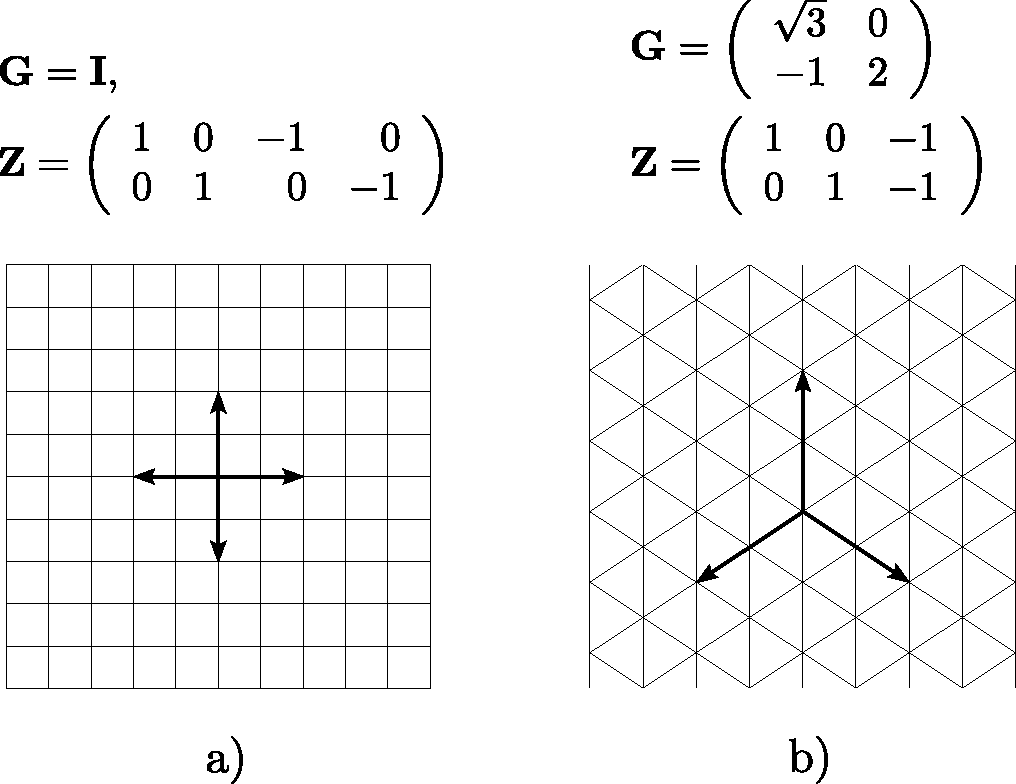
\includegraphics[width=0.70\textwidth]{figures/gps.pdf}
	\caption{Examples of search directions and meshes in $\mathbb{R}^2$ with
		obtained by different choices of $\mathbf{G}$ and~$\mathbf{Z}$. The mesh points
		are at the intersections of the lines, the arrows represent possible search directions.}
	\label{fig:gps}
\end{figure}


After initializing the necessary starting parameters, each iteration of the GPS algorithm is divided into two main steps. The first step is called the search step. During the search step, a finite set $S_k$ of candidate mesh points, selected according to a strategy specified by the user, is evaluated by computing the objective function at each one of the points. If none of the evaluated points represents an improvement over the value $ f(\vec{x}_k) $, the poll step follows. In the poll step, the objective function is evaluated at all neighboring mesh points of $ \vec{x}_k $. The poll set in $k$-th iteration is defined as $P_k = \{x_k + \delta_k d \, | \, d \in \mathbf{D}\}$. If none of the evaluated points represents an improvement over the value $ f(\vec{x}_k) $, we set $ \vec{x}_{k+1} = \vec{x}_k $ and decrease the mesh size, i.e., $ \delta_{k+1} < \delta_k $. However, if a point that improves the estimate of the solution is found in either the search or the poll step, this point is set as $ \vec{x}_{k+1} $, and the mesh size is increased, i.e., $ \delta_{k+1} > \delta_k $~\cite{BBO-textbook, Audet2002}.

The changes described above define a new mesh $ \mathbf{M} _k $ in each iteration. The mesh changes throughout the GPS algorithm. The algorithm terminates when $ \delta_{k+1} < \varepsilon $ for some user-specified $ \varepsilon > 0 $. It can be shown that the mesh step converges to zero, and under appropriate assumptions, the solution estimates converge to a stationary point of the objective function. Details can be found in \cite{BBO-textbook}. It should be noted that the convergence of GPS has been proven for unconstrained problems \cite{BBO-textbook}. The full GPS algorithm is presented in Algorithm~\ref{GPS-algo}.
\\[4pt]
\todo[inline]{Explain what is $t$ and $\tau$ in the algorithm, add typical ranges for $\tau$ maybe.}
\begin{algorithm}[H]
	\caption{Generalized Pattern Search (GPS) for unconstrained optimization}\label{GPS-algo}
	\begin{algorithmic}[1]
		\Require Function $f: \mathbb{R}^n \to \mathbb{R}$, initial point $x_0$, initial mesh size parameter $\delta_0$, positive spanning matrix $\mathbf{D}$, mesh size adjustment parameter $\tau \in (0, 1)$, stopping tolerance $\epsilon_{\text{stop}}$, iteration counter $k \gets 0$
		\Ensure Approximate optimal solution $\vec{x^{\star}}$ for function $f$
		
		\Procedure{GPS}{$x_0$}
		
		\While{$\delta_k > \epsilon_{\text{stop}}$}
		
		\Algphase{1. Search}
		\State Define a finite subset $S_k$ of the mesh $\mathbf{M}_k$
		\If{$f(t) < f(x_k)$ for some $t \in S_k$}
		\State Set $x_{k+1} \gets t$ and $\delta_{k+1} \gets \tau^{-1} \delta_k$
		\State \textbf{continue}
		\Else
		\State Go to Poll step
		\EndIf
		
		\Algphase{2. Poll}
		\State Select a positive spanning set $\mathbf{D}_k \subseteq \mathbf{D}$
		\State Define $P_k = \{x_k + \delta_k d : d \in \mathbf{D}_k\}$
		\If{$f(t) < f(x_k)$ for some $t \in P_k$}
		\State Set $x_{k+1} \gets t$ and $\delta_{k+1} \gets \tau^{-1} \delta_k$
		\Else
		\State $x_k$ is a mesh local optimizer
		\State Set $x_{k+1} \gets x_k$ and $\delta_{k+1} \gets \tau \delta_k$
		\EndIf
		
		\Algphase{3. Termination}
		\If{$\delta_{k+1} \leq \epsilon_{\text{stop}}$}
		\State \textbf{terminate}
		\Else
		\State Increment $k \gets k+1$ and continue
		\EndIf
		
		\EndWhile
		\EndProcedure
	\end{algorithmic}
\end{algorithm}

We turn our attention to the MADS algorithm, which generalizes the GPS algorithm by allowing for a different set of polling directions. The key difference is that MADS introduces the concept of a frame, which allows the poll directions to form a dense subset in $ \mathbb{R}^{n} $ as the algorithm progresses~\cite{BBO-textbook, derivative-free-review}. The frame $\mathbf{F}_k$ at iteration $k$ is defined as
\begin{equation}
	\mathbf{F}_k = \{ \vec{x} \in \mathbf{M}_k \ \big| \ \| \vec{x} - \vec{x}_k \|_\infty \leq \Delta_k b \},
\end{equation}
where $M_k$ represents the current mesh, $ \Delta_k $ is the frame size parameter, satisfying $ \delta_k \leq \Delta_k $, and $b = \max \ \{ \| d \| _\infty \ \big| \ d \in \mathbf{D} \}$. The extent of the frame is determined by the parameter $ \Delta_k $, and the polling directions are taken from this frame.

Each iteration of the MADS algorithm begins similarly to GPS, with a search step where a finite set $S_k$ of candidate points, selected based on the current mesh, is evaluated by computing the objective function at each of the points. If none of these points improves upon the current best solution, the algorithm proceeds to the poll step. 
 
The poll set $P_k$ is a subset of points selected from $\mathbf{F}_k$ and $\mathbf{M}_k$. Trivially, $P_k \subseteq \mathbf{F}_k \subseteq \mathbf{M}_k$. Importantly, the mesh size parameter $ \delta_k $ is allowed to decrease more rapidly than the  enabling the poll directions to asymptotically become arbitrarily dense~\cite{Audet2006}. This aspect is crucial, as it ensures that MADS can explore directions in a finer and more systematic manner than GPS, leading to better convergence properties.


\begin{figure}[H]
	\centering
	\vspace{0.5cm}
	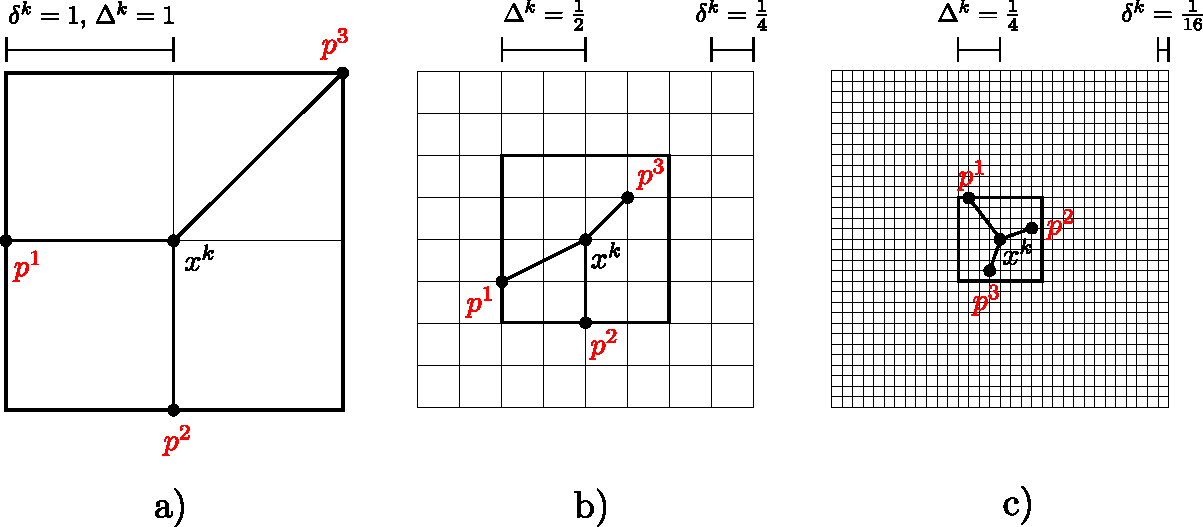
\includegraphics[width=1.01\textwidth]{figures/mads.pdf}
	\caption{Examples of meshes and frames $\mathbb{R}^2$ for different
		values of $\delta_k$ and $\Delta_k$}
	\label{fig:mads}
\end{figure}

If an improvement is found in the poll step, the new point is set as $ \vec{x}_{k+1} $, and the frame size $ \Delta_k $ and mesh size $ \delta_k $ may be increased to encourage further exploration. Conversely, if no improvement is found, $ \vec{x}_{k+1} = \vec{x}_k $, and the mesh size is reduced, i.e., $ \delta_{k+1} < \delta_k $, to allow for a more local search. The process of shrinking and refining the frame and mesh sizes continues until $ \delta_k $ falls below a user-specified threshold, at which point the algorithm terminates.

MADS also incorporates the \textit{extreme barrier function} to handle constraints, similarly to GPS. For constrained optimization problems, the objective function is modified into an extreme barrier function~\cite{BBO-textbook}, which penalizes any infeasible points by assigning them an infinite objective value. This simple yet effective strategy ensures that the optimization remains focused on feasible regions of the search space, and the algorithm converges to a stationary point even for constrained problems. A full description of the MADS algorithm and its implementation details can be found in~\cite{BBO-textbook}.



\begin{algorithm}[H]
	\caption{Mesh Adaptive Direct Search (MADS) for constrained optimization}\label{MADS}
	\begin{algorithmic}[1]
		\Require Function $f_{\infty}: \mathbb{R}^n \to \mathbb{R} \cup \{\infty\}$, initial point, initial frame size parameter $\Delta_0$, positive spanning matrix $\mathbf{D}$, mesh size adjustment parameter $\tau \in (0,1)$, stopping tolerance $\epsilon_{\text{stop}}$, iteration counter $k \gets 0$
		\Ensure Approximate optimal solution $\vec{x^{\star}}$ for function $f$
		
		\Procedure{MADS}{$x_0$}
		
		\While{$\Delta_k > \epsilon_{\text{stop}}$}
		
		\Algphase{1. Parameter Update}
		\State Set the mesh size parameter $\delta_k = \min \{\Delta_k, (\Delta_k)^2\}$
		
		\Algphase{2. Search}
		\State Define a finite set $S_k \subset \mathbf{M}_k$ such that:
		\If{$f_{\infty}(t) < f_{\infty}(x_k)$ for some $t \in S_k$}
		\State Set $x_{k+1} \gets t$ and $\Delta_{k+1} \gets \tau^{-1}\Delta_k$
		\State \textbf{continue}
		\Else
		\State Go to Poll step
		\EndIf
		
		\Algphase{3. Poll}
		\State Select a positive spanning set $\mathbf{D}_{k}$ and define:
		\State $P_k = \{x_k + \delta_k d : d \in \mathbf{D}_{k}\}$, a subset of the frame $\mathbf{F}_k$ with extent $\Delta_k$
		\If{$f_{\infty}(t) < f_{\infty}(x_k)$ for some $t \in P_k$}
		\State Set $x_{k+1} \gets t$ and $\Delta_{k+1} \gets \tau^{-1}\Delta_k$
		\Else
		\State Set $x_{k+1} \gets x_k$ and $\Delta_{k+1} \gets \tau\Delta_k$
		\EndIf
		
		\Algphase{4. Termination}
		\If{$\Delta_{k+1} \leq \epsilon_{\text{stop}}$}
		\State \textbf{terminate}
		\Else
		\State Increment $k \gets k+1$ and continue
		\EndIf
		
		\EndWhile
		\EndProcedure
	\end{algorithmic}
\end{algorithm}
\subsection{Optimization Using a Surrogate Model}\label{model-based}
In cases where evaluating the objective function at a specific point is time-consuming or computationally expensive, it can be useful to employ a surrogate model for the objective function during optimization. We define a surrogate model of the given problem as the problem

\begin{equation}
	\min_{\vec{x} \in \mathbf{\tilde{X}}} \tilde{f}(\vec{x}),
\end{equation}
where
\begin{equation}
	\mathbf{\tilde{X}} = \left\{ \vec{x} \in \mathbf{D} \subseteq \mathbb{R}^n \ \middle| \ \vec{\tilde{g}} (\vec{x}) \leq \vec{0} \wedge \vec{\tilde{h}} (\vec{x}) = \vec{0} \right\},
\end{equation}
and the functions \( \tilde{f}, \vec{\tilde{g}} \), and \( \vec{\tilde{h}} \) have characteristics similar to those of the functions \( f, \vec{g} \), and \( \vec{h} \) in the original problem. The characteristics of \( \tilde{f}, \vec{\tilde{g}} \), and \( \vec{\tilde{h}} \) are intentionally left undefined, reflecting the fact that the surrogate model does not necessarily need to be an accurate approximation of the original problem \cite{BBO-textbook, two-decades, Kramer2011}. A good approximative model may not always be a suitable surrogate for optimization purposes, a situation illustrated in Figure \ref{fig:surrogate}.

\begin{figure}[H]
	\centering
	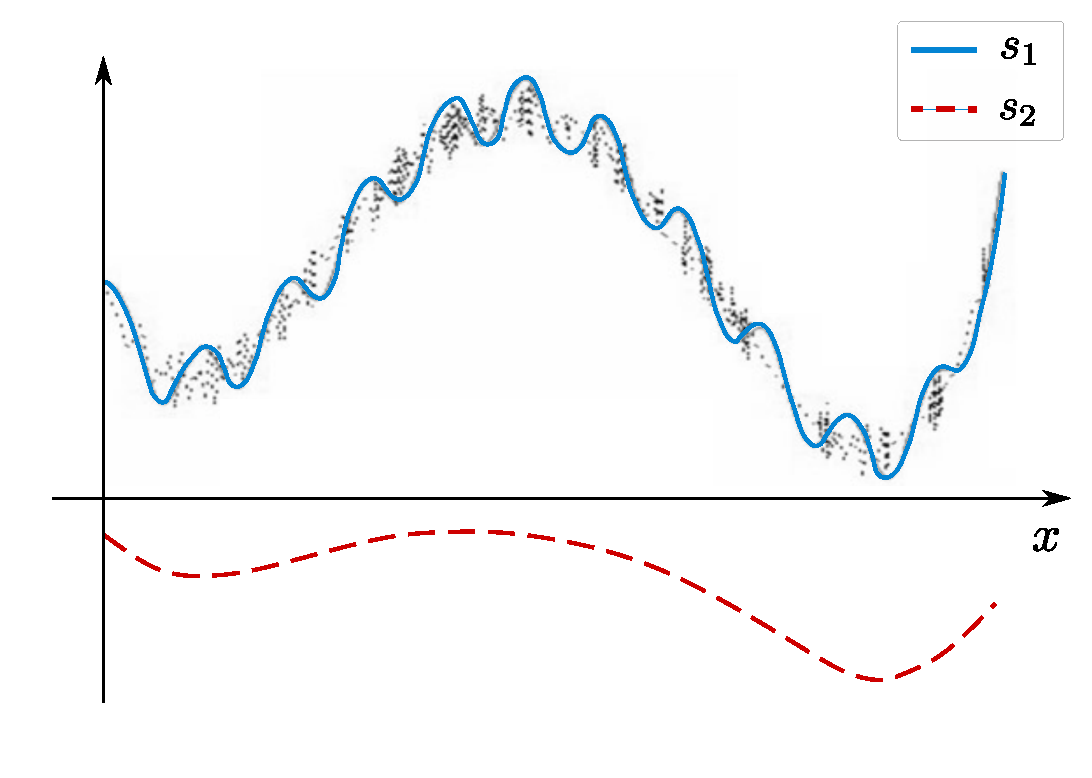
\includegraphics[width=0.6\textwidth]{figures/surrogate.pdf}
	\caption{An illustration of two surrogate models, $ s_1 $ and $ s_2 $. The black points represent noisy values of the objective function. While using surrogate model $ s_1 $ represents a better choice for approximating the function, it is not suitable for optimization since $ s_1 $ contains many undesirable stationary points that the original objective function does not have. On the other hand, while surrogate model $ s_2 $ is not as accurate in approximating the function's values, it is a better choice for optimization because the stationary points of $ s_2 $ are almost identical to those of the optimized objective function.}
	\label{fig:surrogate}
\end{figure}

Using a surrogate model in optimization is often just a part of a more complex optimization method. Surrogate models can, for example, be used within GPS and MADS methods described in section \ref{direct-search}, where, during the poll step, we first evaluate the surrogate function \( \tilde{f} \) at the points from the poll set, sort these values, and use them to sort the poll set used to evaluate the original function \( f \). This potentially allows us to significantly reduce the time required to complete the poll step, as sorting the points increases the probability of finding a better estimate of the solution at one of the first examined points \cite{BBO-textbook}. Surrogate models can also be used within other methods to accelerate the optimization process, and their application is discussed in detail in \cite{BBO-textbook, two-decades}.

\section{Description of the optimization framework}\label{framework}
A fully automated and modular optimization framework was developed to solve the optimization problems in this work. The proposed framework is composed of several components, which are described in detail below:

\begin{enumerate}
	\item \textbf{Optimization}:  
	The first component encompasses the optimization method, which governs the entire process. In this part, the optimization problem is defined along with any required constraints.
	
	In this study, we use the Nelder-Mead method, implemented in Python specifically for this work and detailed in Appendix~\ref{appendix B}. Additionally, the framework includes the MADS method (see Section~\ref{direct-search}), implemented in the open-source \texttt{NOMAD} library \cite{nomad} in C++. For handling constraints in both the Nelder-Mead and MADS methods, we use the extreme barrier function.
	
	\item \textbf{Geometry Generation}:  
	The optimization parameters, updated at each iteration, are passed to the geometry generator. For generating the geometries used in numerical simulations, we use the \texttt{meshgen} package detailed in Chapter~\ref{geometry}.
	
	\item \textbf{Numerical Simulation}:  
	The final component of the optimization framework is the numerical solver, which evaluates the objective function based on the generated geometry. Numerical simulations are performed using the LBM, which is described alongside additional implementation details in Chapter~\ref{lbm}.
\end{enumerate}

The interconnection of these components within the optimization framework is schematically illustrated in Figure~\ref{fig:framework}.


\begin{figure}[H]
	\vspace{5mm}
	\centering
	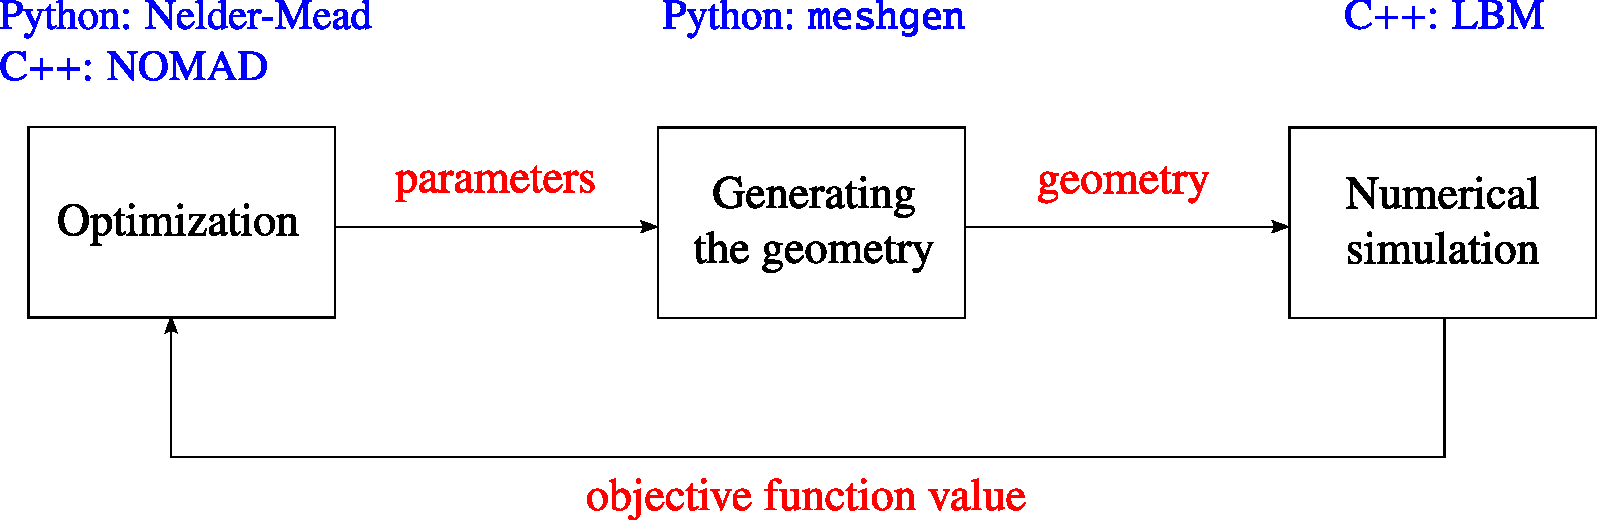
\includegraphics[width=0.95\textwidth]{figures/framework-en.pdf}
	\vspace{5mm}
	\caption{Schematic representation of the modular optimization framework. It consists of three main components: (1) Optimization, which defines the problem and governs the iterative process, (2) Geometry generation, where optimization parameters are translated into geometric models using \texttt{meshgen}, and (3) Numerical simulation, where the objective function is evaluated using the LBM.}
	\label{fig:framework}
	
\end{figure}
